\chapter{Numerical simulation of two flash flood events in the UK}
\label{chapter_events}
\chaptermark{Severe storms in Cornwall and northern England}

\section{Background}
Intense rainfall events may be short lived, lasting only a few hours, but have the potential to cause substantial and destructive flooding \citep{lane2008climate,pitt2008pitt}. In the UK, many of these storms occur in the summer \citep{Kendon2014}, and their severity is often the result of a combination of meteorological factors. From a meteorological perspective, flash flooding can be predicted through an ingredients-based method; a systematic assessment of the key components present to cause an intense rainfall event likely to lead to flash flooding \citep{Doswell1996}. In the ingredients-based approach, flash flooding occurs when there is a combination of a high rainfall rate for an extended duration of time (usually on the order of hours). Rainfall totals are in turn related to the length of the rainfall event. Factors that lead to high rainfall intensity during an event include the forced ascent of moist air, usually associated with orographically-forced rainfall events \citep{Barros1994,Houze2012}. The duration of the event is dependent of the speed of movement and the size of the system bringing rainfall; given equal intensity rainfall rates, a large, slow moving rainfall feature will cause much higher rainfall totals in a river catchment that a fast moving, smaller feature. 

Though not essential to the `ingredients-based' method of flash flood prediction, convective-type storms are frequently associated with the type of intense rainfall that leads to flash flooding \citep{doswell1993flash}, including highly-localised flooding in the UK \citep{gray1998mesoscale,Browning2007}. In certain cases, convective rainfall events may appear stationary or `quasi-stationary' \citep{chappell1986quasi,warren2014boscastle}, leading to prolonged intense rainfall over river catchments.

The combination of these ingredients leads to river catchments being subjected to high-intensity rainfall inputs at a rate faster than a river catchment can transport or store water, leading to river flooding when rivers exceed their bankfull\footnote{The water level at which a river is at the top of its banks and any further rise would result in water moving into the flood plain.} capacity, or surface water flooding if rainfall rates are greater than infiltration rates at the surface. Antecedent conditions, such as soil-moisture content, also play a role in a catchment's ability to store water, but in cases of the most extreme rainfall events, even catchments with a high potential to store incoming rainfall or slow water flow towards rivers will be overwhelmed with the rate and volume of water input and flooding becomes inevitable.

This chapter describes two intense rainfall and flash flooding events in the UK summers of 2004 and 2005. The cause and impact of the events are described as a background to them being used as case studies in a series of numerical simulations. The series of numerical simulation experiments are designed to investigate the role of rainfall spatial resolution in hydrological and geomorphological processes during severe storms, as described in Chapter \ref{chapter_intro}. % Extension from the intro chapter?

The two events used as case studies took place in 1) the Ryedale catchment, near the town of Helmsley, North Yorkshire, 2005; and  2) the Valency catchment near the village of Boscastle, Cornwall, 2004. Both catchments experienced intense rainfall leading to extensive and damaging flash flooding \citep{golding2005boscastle,sibley2009analysis}. There were significant economic impacts for both communities, as well as geomorphological changes to the river channels and flood plains observed in the aftermath of the flooding \citep{wallingford2005flooding,wass2008investigation}.

\section{Meteorological setting}
The case studies were chosen as they represented infrequent events in each particular catchment. Because there is no commonly agreed definition of what constitutes an extreme or infrequent event \citep[e.g.][]{wilby2008climate,fowler2010detecting,jones2014objective,}, for the purpose of this study, flood events likely omly to occur approximately once in several hundred years were chosen. (The return period for the 3 hour rainfall event is given in Table \ref{table_met_setting}.) Peak river discharges for each of the case study flood events exceeded the 99th percentile for their respective catchments \citep{hannaford2004development,NRFA}.  An overview map of the catchment locations is given in Figure \ref{fig_location_map}, marked by the location of their main settlements. Table \ref{table_met_setting} summarises the key features of each catchment and its associated storm.

\begin{figure}[htb]
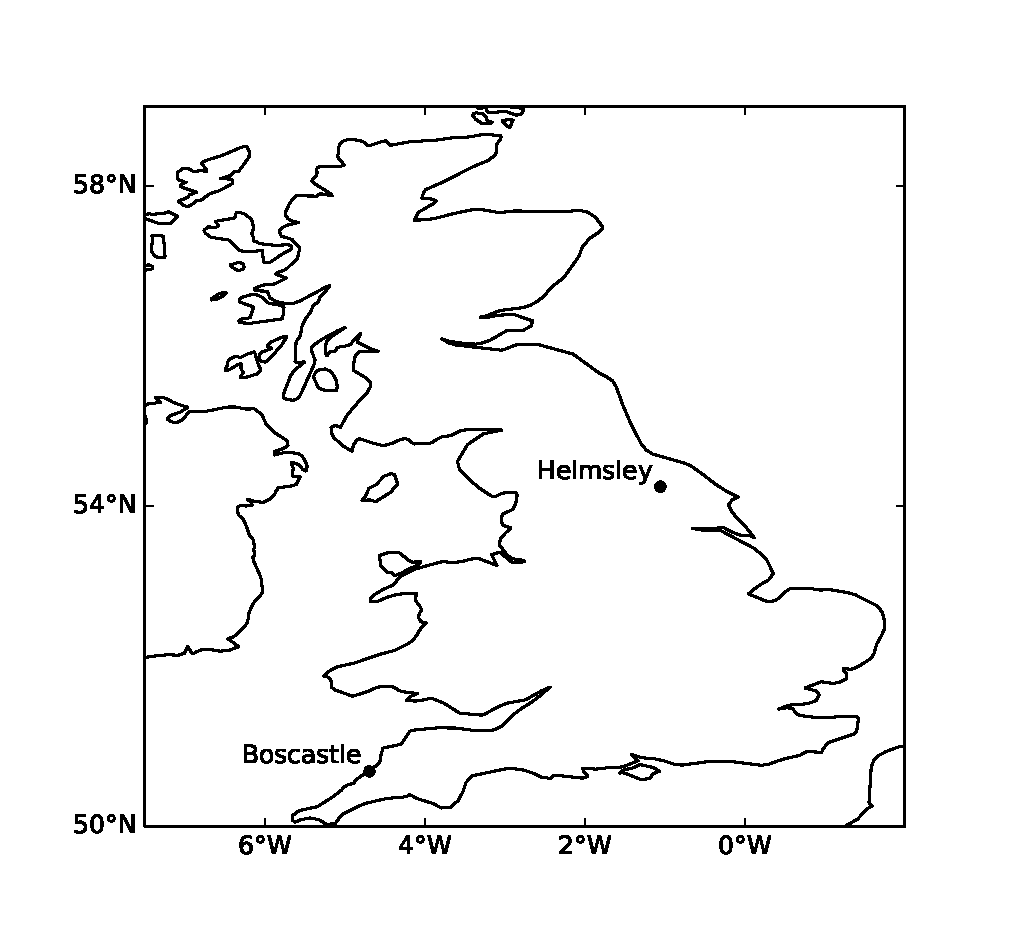
\includegraphics[width=11cm]{chp_events_figures_scripts/figure_location_map.eps}
\caption{Location of the two case study catchments in Britain, marked by the main settlement within each catchment.}
\label{fig_location_map}
\end{figure}

\linespread{1.5}
\begin{table}
\resizebox{\textwidth}{!}
{%
\begin{tabular}{l c c} \hline

Catchment Name 			& \textbf{Ryedale} &  \textbf{Valency} \\ \hline
Main settlement        & Helmsley             & Boscastle \\
Catchment Area   			& 270km$^2$ 				& 18km$^2$ \\ 
Catchment Type         & Upland, Moor/Peaty & Upland, Pasture \\ 
Storm Date	 		            & 2005-06-19 	& 2004-08-16 \\ 
Peak Rainfall	 (mm hr \(^{-1}\))  & 125  & c.400 \\
%Peak Discharge	 	 & & \\ 
Meteorological Setting	 	& Split-front, convective system & Quasi-stationary convective system \\ 
3hr Rainfall Return Period 	 & 330yr \citep{wass2008investigation}	& 1300yr \citep{burt2005cloudburst} \\ \hline
\end{tabular}
}
\caption{Table showing key characteristics of each storm event.}
\label{table_met_setting}
\end{table}

\subsection{Boscastle, Cornwall storm 2004}
The Boscastle storm took place on 16 August 2004. The storm led to flooding within the River Valency catchment and the village of Boscastle. In the preceding months March--June, the south-west area of Britain had been drier than usual, although during July the Valency catchment area experienced average rainfall conditions \citep{golding2005boscastle}. The estimated soil moisture deficit\footnote{The amount of water needed to bring the soil back to field capacity, i.e. a state where the soil is holding the maximum amount of water possible against gravity. \citep{beven2011rainfall}} in the area, which had previously been lower than average due to the dry antecedent conditions in March--June, decreased during 1--16 August, due to a return to average rainfall conditions in that month. The soil moisture deficit during this period was estimated to have decreased from approximately 80--220mm to 40--180mm \citep{golding2005boscastle}.

On the day of the storm, rainfall accumulations of up to 184mm from the Lesnewth tipping bucket raingauge \citep{golding2005boscastle} were recorded in the upper Valency catchment resulted from prolonged rainfall between 1200--1600 UTC. Rainfall rates were thought to have reached almost 400 mm hr\(^{-1}\) \citep{golding2005boscastle}, after correcting for under-reporting from rain gauges in the vicinity of the catchment \citep{burt2005cloudburst}. The rainfall accumulations from the 1km gridded composite radar product in the Valency catchment are shown in Figure \ref{fig_boscastle_rain_totals}. Note that the highest rainfall accumulations from the radar data shown in Figure \ref{fig_boscastle_rain_totals} are 115mm, lower than the raingauge totals reported in \citet{golding2005boscastle}, likely due to under reporting by precipitation radar. 

%The meteorological conditions that enabled such prolonged heavy rainfall were a combination of large-scale synoptic conditions moving in from the Atlantic, with moist lower atmospheric layers readily forming convective cloud. Repeated initiation of convection along the north Cornish coast lead to what appeared to be relative stationary convective cells over the Valency catchment. Later authors refer to this type of convective storm as a `Boscastle-type' or quasi-stationary convective storm \citep{warren2014boscastle}.

\begin{figure}[htb]
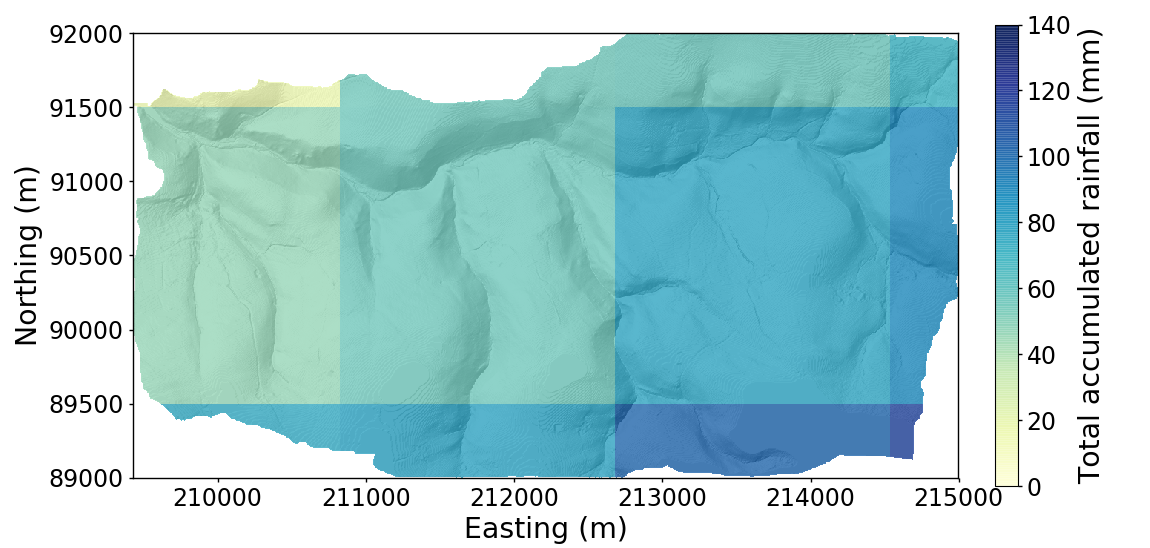
\includegraphics[width=15cm]{chp_events_figures_scripts/figure_boscastle_total_rainfall.png}
\caption{Total accumulated radar rainfall (24 hours) over the Valency (Boscastle) catchment during the 16th August 2004.}
\label{fig_boscastle_rain_totals}
\end{figure}


\subsection{Ryedale, North York Moors storm 2005}
The Ryedale storm occurred on 19 June 2005. Intense rainfall throughout the afternoon led to total accumulated rainfall amounts of up to 89mm in Ryedale between 1400--1800 UTC measured by the Helmsley raingauge. Peak instantaneous rainfall rates were estimated to have been around 32.5mm hr\(^-1\) \citep{sibley2009analysis} to 59.4 mm hr\(^{-1}\) \citep{hopkins2012knowledge}, though one report states they reached as high as 125 mm hr\(^{-1}\) \citep{cinderey2005north}. Figure \ref{fig_ryedale_rain_totals} shows the total accumulate rainfall radar totals from the 1km composite radar product. Most areas of the catchment received total rainfall accumulations similar to the reported raingauge figure (89mm), though up to 131mm is reported in one grid square in the south of the catchment area.

Antecedent conditions before the Ryedale storm of 2005 were dry over a prolonged period over much of the region \citep{sibley2009analysis}, leading to cracking of the surface peat in the higher elevations of the catchment. Soil moisture deficit was estimated to be around 60mm in the catchment, higher than usual due to the drier conditions in the preceding months \citep{wass2008investigation}. With a high soil moisture deficit, thinner soils in the upper reaches of the catchment would have been dry before the intense rainfall.

%The meteorological conditions leading to such heavy rainfall was a combination of a cold, upper-level air mass advecting over a warm moist boundary layer, leading to unstable conditions that enabled a convective thunderstorm to develop in the late afternoon. The conditions let to a particularly high amount of precipitable water present in the atmosphere which was subsequently washed out into the landscape during intense rainfall. 

\begin{figure}[htb]
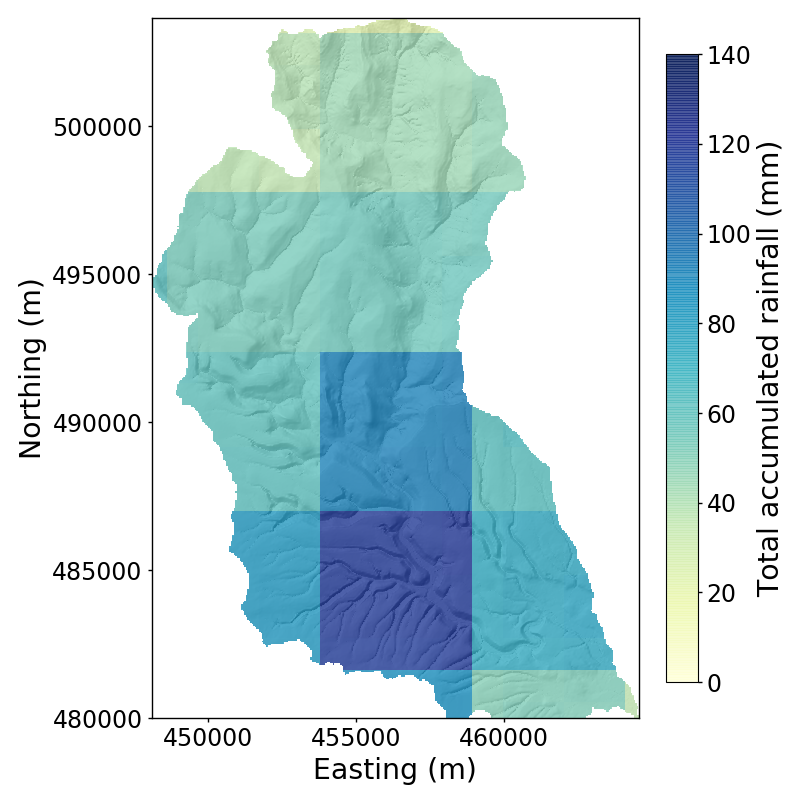
\includegraphics[width=13cm]{chp_events_figures_scripts/figure_ryedale_total_rainfall.png}
\caption{Total accumulated radar rainfall (24 hours) over the Ryedale catchment during the 19th June 2005.}
\label{fig_ryedale_rain_totals}
\end{figure}

\section{Flooding and geomorphic change}

\subsection{Boscastle, Cornwall, 2004}
Flooding was extensive in the area surrounding Boscastle village, with flood levels rapidly exceeding bankfull and flooding several properties to depths of several metres. Water levels in the Valency river and its tributaries began to rise in the early afternoon from approximately 1200 UTC onwards, reaching bankfull around 1430 UTC and peaking at around 1600 UTC, by which point over 70 properties had been flooded, with several destroyed due to the force of the water \citep{wallingford2005flooding}.

The routing of flood waters in the Boscastle flood was complicated due to the role of large debris blockages (`trash barriers') in the river channels. In particular, a large debris blockage formed under the main bridge in the village crossing the Valency, which caused a significant backup of water behind the bridge, and re-routing of water through alternate pathways within the village. A reconstruction of the flood based on eyewitness accounts and water mark levels consequently resulted in different reports of the peak water level in the village depending on where the observations were made \citep{wallingford2005flooding}. 

The geomorphological impacts of the flood event were well documented in the aftermath of the event \citep{wallingford2005flooding}. The Valency river channel and many of its tributaries experienced channel avulsion\footnote{Movement of the original channel to a new position within the flood plain.} in places, as well as significant downcutting in the upper tributary channels of the catchment. In a number of places the channel avulsion was substantial enough to straighten the channel and increase the local gradient of the river, potentially increasing flow velocities and shear stresses acting on the channel bed. There were large amounts of sediment observed in the river flow at the time, ranging in size from fine silts to boulders. There were some areas of sediment deposition observed along the river channel banks and floodplain, and a sizeable area of sediment deposition in Boscastle harbour. However, most stretches of the main river channel and its tributaries showed net erosion in the form of channel widening (up to 3--4 metres) and deepening (of up to 2 metres) \citep{wallingford2005flooding}.

\subsection{Ryedale, North Yorkshire, 2005}
Flooding was widespread in the Ryedale catchment, with river levels reaching up to 3.5m at Hawnby, a smaller settlement upstream of Helmsley. At the peak of the flood, the Hawby gauging station building was completely submerged\citep{wass2008investigation}. In Helmsley, the largest settlement, further downstream, similar river level rises of up to 2m were reported at the peak of the flood in the evening and into the night. 

Geomorphologically, the Ryedale catchment saw relatively rapid change considering the short duration of the storm and subsequent flood on 19 June. In the aftermath of the flood, up to 2--3 metres of channel downcutting and erosion were reported to have take place in the upper reaches of the tributaries of the catchment \citep{hopkins2012knowledge,wass2008investigation} as well as significant amounts of sediment and debris deposition in the lower reaches of the catchment around Helmsley \citep{hopkins2012knowledge}. The storm triggered many landslides on hillslopes within the catchment, including 105 reported shallow landslides in the catchment, as well as two large peat slides in moorland areas covering up to 3.7 ha of mass movement in areal extent \citep{galiatsatos2007assessment,wass2008investigation}. Dry antecedent conditions in the area are believed to have been a main cause of landsliding in the area by weakening the peat moorland within the catchment \citep{sibley2009analysis}. Dry conditions preceeding summer storms can cause shrinkage and cracking in peatlands, leading to greater risk of erosion in heavy downpours \citep{warburton2004hydrological}. 
The economic damage was also substantial for a sparsely populated area. Three bridges were destroyed at a cost of £2.9 million, as well as flooding of 121 properties \citep{wass2008investigation}. Economic loss included agricultural damage such as loss of land and livestock \citep{sibley2009analysis}. Many residents were displaced for months during repair and were reported to have suffered illness and psychological trauma from the event \citep{hopkins2012knowledge}.



\section{Experiment design}
\label{section_experiment_design}

Using the two flash flood events described previously as case studies, an ensemble of simulations was designed to address the questions laid out in Chapter \ref{chapter_intro} and summarised in the following hypotheses:

\begin{enumerate}

\item \label{itm:flood} \textbf{Flood inundation modelling is sensitive to the spatial detail of precipitation inputs.}
  \begin{enumerate} 
  \item \label{itm:hydro} Catchment hydrology is sensitive to the spatial distribution of rainfall inputs over the catchment area. Resolving the spatial details of a precipitation event, such as during a flash flood, allows the timing and magnitude of flood inundation to be better predicted.
  \item Geomorphological change of the river channel and flood plain during a flash flood is substantial enough to alter the patterns of flood inundation. In a model that can account for erosional change during flooding, nuances in flood inundation can be better predicted.
  \end{enumerate}

\item \label{itm:geomorph} \textbf{Erosional processes in river catchments are sensitive to the spatial distribution of rainfall inputs.}
  \begin{enumerate}
  \item Erosion and sediment transport processes are sensitive to thresholds determining erosion initiation and sediment entrainment. If item (\ref{itm:hydro})  holds true, then fluvial erosional processes should exhibit sensitivity to the spatial distribution of rainfall inputs of rainfall as well.
  \item The parameterisation of erosional processes in the model also determines the spatial pattern of erosion and deposition, but does spatial variation in rainfall inputs exert a greater control than the choice of erosion law?
  \end{enumerate}
  
\end{enumerate} 

To test the above hypotheses, simulations of the two case studies were repeated, varying the following conditions:

\begin{itemize}
\item Rainfall spatial resolution: 1km-gridded/uniform
\item Erosion law: transport-limited/detachment-limited
\end{itemize}

The simulations were parameterised with different erosion law schemes and different rainfall input resolutions to assess which factor exerted the greatest control over flood inundation and sediment transport within the catchment. The same set of experiments was carried out for both the Boscastle and Ryedale events, giving a total of 6 different simulations for each catchment outlined in Table \ref{table_ensemble_experiments} -- a total of 12 simulations.

\begin{table}
\begin{tabular}{lll}
\\
\textbf{Experiment name}   & \textbf{Rainfall input} & \textbf{Erosion law}  \\
\hline
UNIFORM\_HYDRO  &  Spatially-averaged  Radar  & (no erosion) \\
UNIFORM\_DLIM      &  Spatially-averaged  Radar & Detachment-limited \\
UNIFORM\_TLIM       &  Spatially-averaged  Radar & Transport-limited \\

GRIDDED\_HYDRO  &  1km Radar Gridded  & (no erosion) \\
GRIDDED\_DLIM      &  1km Radar Gridded  & Detachment-limited \\
GRIDDED\_TLIM       &  1km Radar Gridded   & Transport-limited \\
\hline \\ 
\end{tabular} 
\caption{Outline of the simulations carried out for both the Ryedale and Boscastle case studies.}
\label{table_ensemble_experiments}
\end{table}

\

\subsection{Model initialisation and configuration}
The numerical landscape evolution model, HAIL-CAESAR was used for all simulations.  The equations describing the water routing, sediment erosion, and transport laws are described fully in Chapter \ref{chapter_HAIL-CAESAR}.
%
%HAIL-CAESAR is a hydrodynamic landscape evolution model that uses a TOPMODEL-based hydrological rainfall-runoff model to generate surface runoff in a river catchment, which is then routed through the landscape according to an adaptation of the LISFLOOD-FP shallow water routing algorithms \citep{bates2010simple}. Fluvial erosion and sediment transport is then derived using the velocities and depths of the calculated surface water within the catchment.

\subsubsection{Input data}
Rainfall input data is taken from the Met Office NIMROD radar rainfall 1km composite dataset \citep{metoffice2003nimrod}. The same 1km rainfall radar product is used to derive the rainfall inputs for the spatially uniform rainfall simulations, by averaging out the gridded rainfall data over the input points of the catchment, thus preserving the total amount of rainfall input in each simulation, and only varying its spatial distribution for the relevant gridded rainfall input simulations.

Topographic data used to initialise the terrain surface for the Boscastle simulation is derived from the Environment Agency (England) 2m LiDAR product. The Boscastle data is resampled to 5m grid spacing to reduce the total number of grid cells and the  computational demands of running a complex hydrodynamic model. Environment Agency LiDAR was not available for the whole Ryedale catchment at the time of the simulation, so the Ryedale terrain is initialised using Ordnance Survey `Terrain 50' data, interpolated to 5m grid spacing to enable like-for-like comparison with the Boscastle terrain grid spacing. Resampling the initial topographic data sources to the same terrain grid spacing of 5m for both sets of simulations is done to minimise the potential effects that variation in grid spacing has on model output and subsequent topographic analysis \citep[e.g][]{chang1991effect,schoorl2000three,haile2005effects,zhang2008effects}

\subsubsection{Simulation duration}

The simulations are set to begin 24 hours before the day of each storm event. The model is allowed to run for a further 24 hours after the event, giving a total simulation time of 72 hours. The timing of the simulations is given in Table \ref{table_start_time_hydrog_sims}.

\begin{table}[htbp]
\begin{tabular}{l c  c}
\textbf{Event}  &   \textbf{Start time} &  \textbf{End time} \\
\hline 
Boscastle          &  2004-08-15 00:00  &  2004-08-17 23:59 \\
Ryedale             &  2005-06-18 00:00  &  2005-06-20 23:59 \\
\hline

\end{tabular}
\caption{Start and end times (UTC) for each 72 hour simulation. The major rainfall event occurs during the second day in each simulation.}
\label{table_start_time_hydrog_sims}
\end{table}

\subsubsection{Rainfall spatial resolution}
In order to assess the sensitivity of hydrogeomorphic processes to the spatial details of precipitation, rainfall spatial inputs were alternated in each simulation between a spatially uniform rainfall input and a 1km gridded rainfall input. Both the spatially uniform and gridded inputs were based on the same original rainfall source data -- the UK Met Office Nimrod 1km-composite radar data product \citep{metoffice2003nimrod}. The uniform rainfall input data were created from averaging out the gridded data in spcae over the model domain. The temporal resolution of the five minute interval data was preserved, giving a time series of spatially averaged rainfall rates for the duration of the each simulation. To reduce the range of variables within the set of ensemble simulations, only the spatial resolution of rainfall was assessed in this study -- other studies had already investigated the effects of the \textit{temporal} resolution of rainfall data on discharge and erosion rates \citep{nicotina2008impact,Coulthard2013,coulthard2016sensitivity}. In all experiments, the temporal resolution of rainfall data was maintained at five minute intervals. To summarise, the two types of rainfall spatial input used were: 

\begin{itemize}
\item Uniform or `lumped' precipitation: Radar-derived rainfall rates across the catchment are spatially-averaged to produce a catchment-wide rainfall rate. In other words, every grid cell in the model domain receives the same rainfall rate at each five minute rainfall data timestep.
\item Gridded rainfall input. The rainfall rate is input from a overlying gridded mesh of raincells, at the same grid spacing as the rainfall radar product (1km).
\end{itemize}

\subsubsection{Erosion-enabled simulations}
A variety of erosion laws exist describing how landscapes erode from fluvial erosion. The choice of erosion law for a given catchment depends on a variety of factors, such as the characteristic substrate material in the catchment -- is it predominantly loose sediment or cohesive, solid bedrock? In reality, many upland landscapes in the UK are often a mixture of these two extremes, incorporating a thin layer of loose sediment on top of solid bedrock. Streams in such landscapes may be termed mixed-channel systems \citep{howard1998long}, and many variants on the fluvial incision laws incorporating the role of sediments have been proposed \citep{Lague2005,sklar2006role}. Catchments also often exhibit a transition from rockier upland headwaters, to more thickly soil-mantled floodplains. In order to address the sensitivity to the choice of erosion model for each event simulation (Chapter \ref{chapter_landscape_evol}), two erosion model end-members are used, with each one representing a different conceptual model of fluvial erosion and sediment transport. These include: i) a purely sediment transport-limited model \citep{wilcock2003surface}, ii) a detachment-limited bedrock erosion model \citep{howard1983channel,stock1999geologic,whipple1999dynamics}. The equations describing the transport-limited and detachment-limited models used in the model are discussed in detail in Chapter \ref{chapter_HAIL-CAESAR}. Further erosion laws were considered, such as a hybrid transport- and detachment-limited erosion model, but it was deemed beyond the scope of this study, which is primarily to investigate the role of rainfall heterogeneity, rather than the wide range of erosion and sediment transport models. In keeping with the primary aim of the study, it was opted to use two simple variants of sediment erosion laws to keep the range of model simulations parsimonious. 

\subsubsection{Flood inundation only simulations}
A set of control simulations (suffixed \textit{HYDRO}, for example in Table \ref{table_ensemble_experiments}) incorporating only rainfall-runoff and surface water routing (with no erosion taking place) were also carried out for comparison against the two erosion end-member simulations. The analysis from these experiments is used to investigate the sensitivity of flood-inundation prediction to geomorphic change during floods, and the results and discussion are presented in Chapter \ref{chapter_flood_model_sensitivity}.

%\paragraph*{Hybrid model}
%The hybrid model assumes a limited-depth sediment layer, overlying a bedrock layer. Figure \ref{hybrid_model} shows a typical cross section through a typical valley in the hybrid model set-up. In the initial model state (before the spin-up period), a channel is 'burnt-in' to the sediment-layer. Whenever bedrock becomes exposed during the hybrid simulation, the simple detachment-limited erosion law is applied. Material removed from the bedrock layer is then apportioned between the various sediment fractions. At all other times, the sediment transport law applies to the sediment layer. 



%\subsubsection{Model spin-up}
%
%The HAIL-CAESAR model (Valters ?\& Coulthard?, 2016/7) initialises the model domain with a uniform distribution of sediment grain sizes across the catchment. This is physically unrealistic, so the model domain is `spun-up' for a simulated time of 1000 days using typical rainfall data for each catchment. This ensures a heterogeneous distribution of sediment throughout the catchment prior to the detailed storm simulations. 

\section{Summary}

Using case studies from two flash flood events in the UK that took place in recent decades, a series of simulations was designed to investigate the effects of rainfall spatial resolution on flood inundation modelling, and sediment erosion and transport. The simulations are designed to answer the questions laid out in Chapter \ref{chapter_intro} and the hypotheses summarised in Section \ref{section_experiment_design}. 

The results and analyses from the simulations are discussed in the subsequent chapters. Chapter \ref{chapter_flood_model_sensitivity} analyses and discusses the effects that rainfall spatial resolution has on flood inundation prediction in the HAIL-CAESAR numerical model, and also looks at the effects that geomorphic change during a flood has on flood dynamics. This addresses Question \ref{itm:flood} laid out in Section \ref{section_experiment_design} above. 

Chapter \ref{chapter_hydrogeomorph} analyses the results of the simulations focusing on sediment erosion and transport, discussing whether the spatial patterns of rainfall control the distribution of erosion and deposition in a catchment. The implications for longer-term landscape evolution modelling are also discussed. Chapter \ref{chapter_hydrogeomorph} addresses Question \ref{itm:geomorph} laid out in Section \ref{section_experiment_design} above. Conclusions and links between rainfall inputs, hydrological, and geomorphological processes are discussed in Chapter \ref{chapter_conclusion}.
